Central to the discussion of solvent is a discussion of how to formulate the surface of a protein.
The most frequently used formulations of surface area include the Van der Waals (VDW) surface, the solvent accessible surface, and the Connolly surface (also known as the molecular surface).
\begin{figure}[h]
\centering
\begin{subfigure}[b]{0.4\textwidth}
\centering
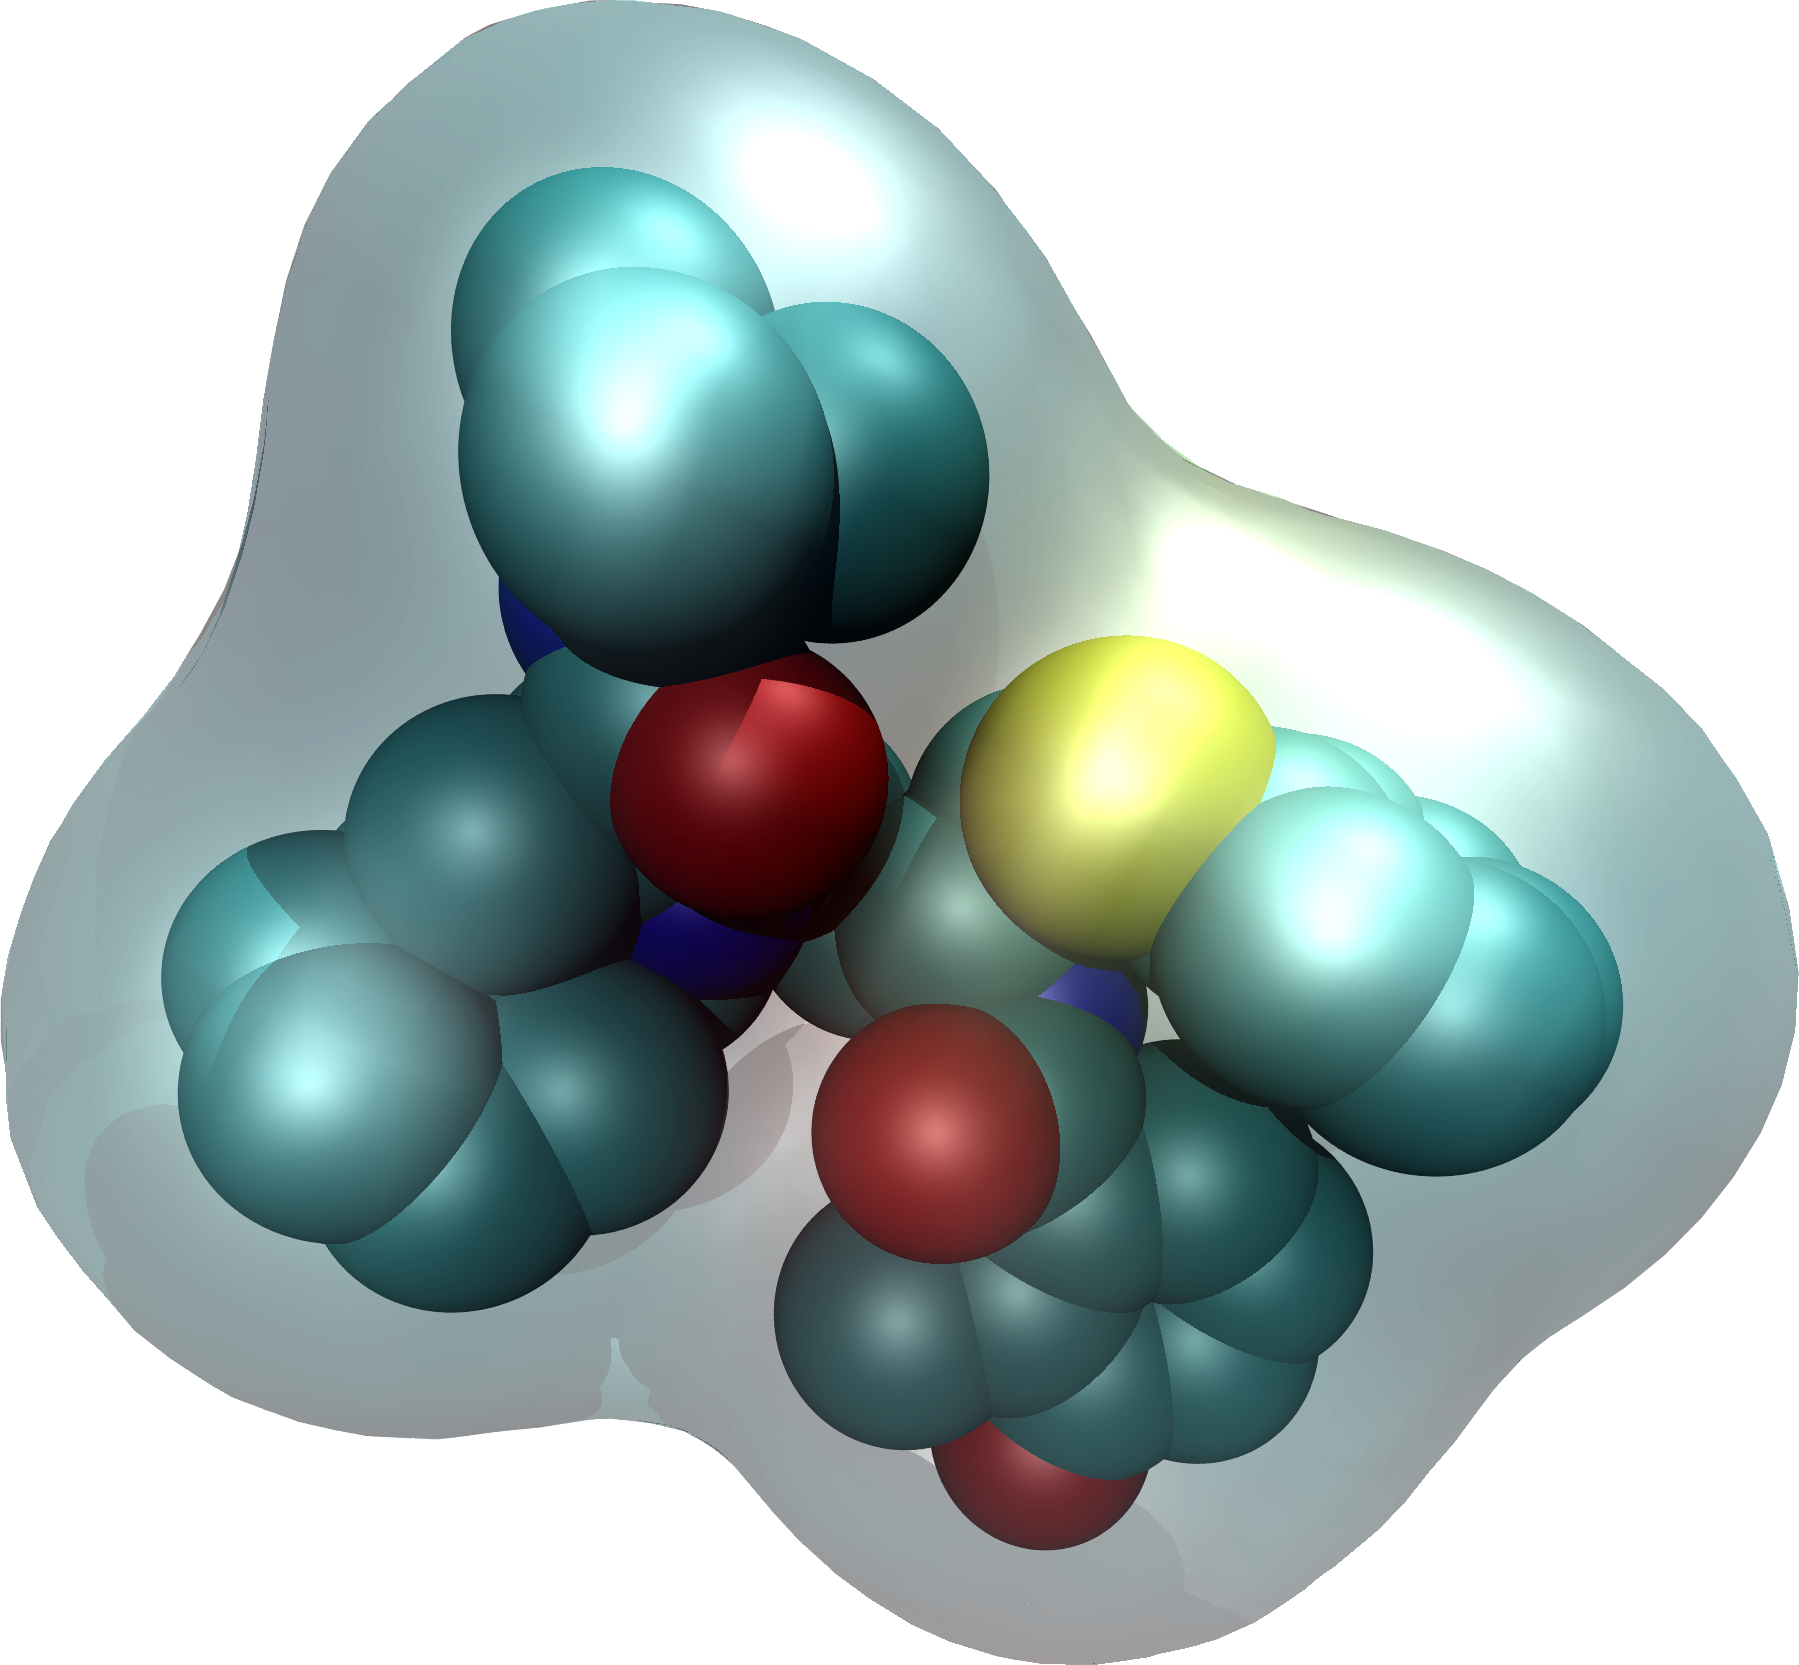
\includegraphics[width=\textwidth]{figures/vdw.png}
\caption{}
\label{figure:vdw_surface}
\end{subfigure}
\hspace{0.1\textwidth}
\begin{subfigure}[b]{0.4\textwidth}
\centering
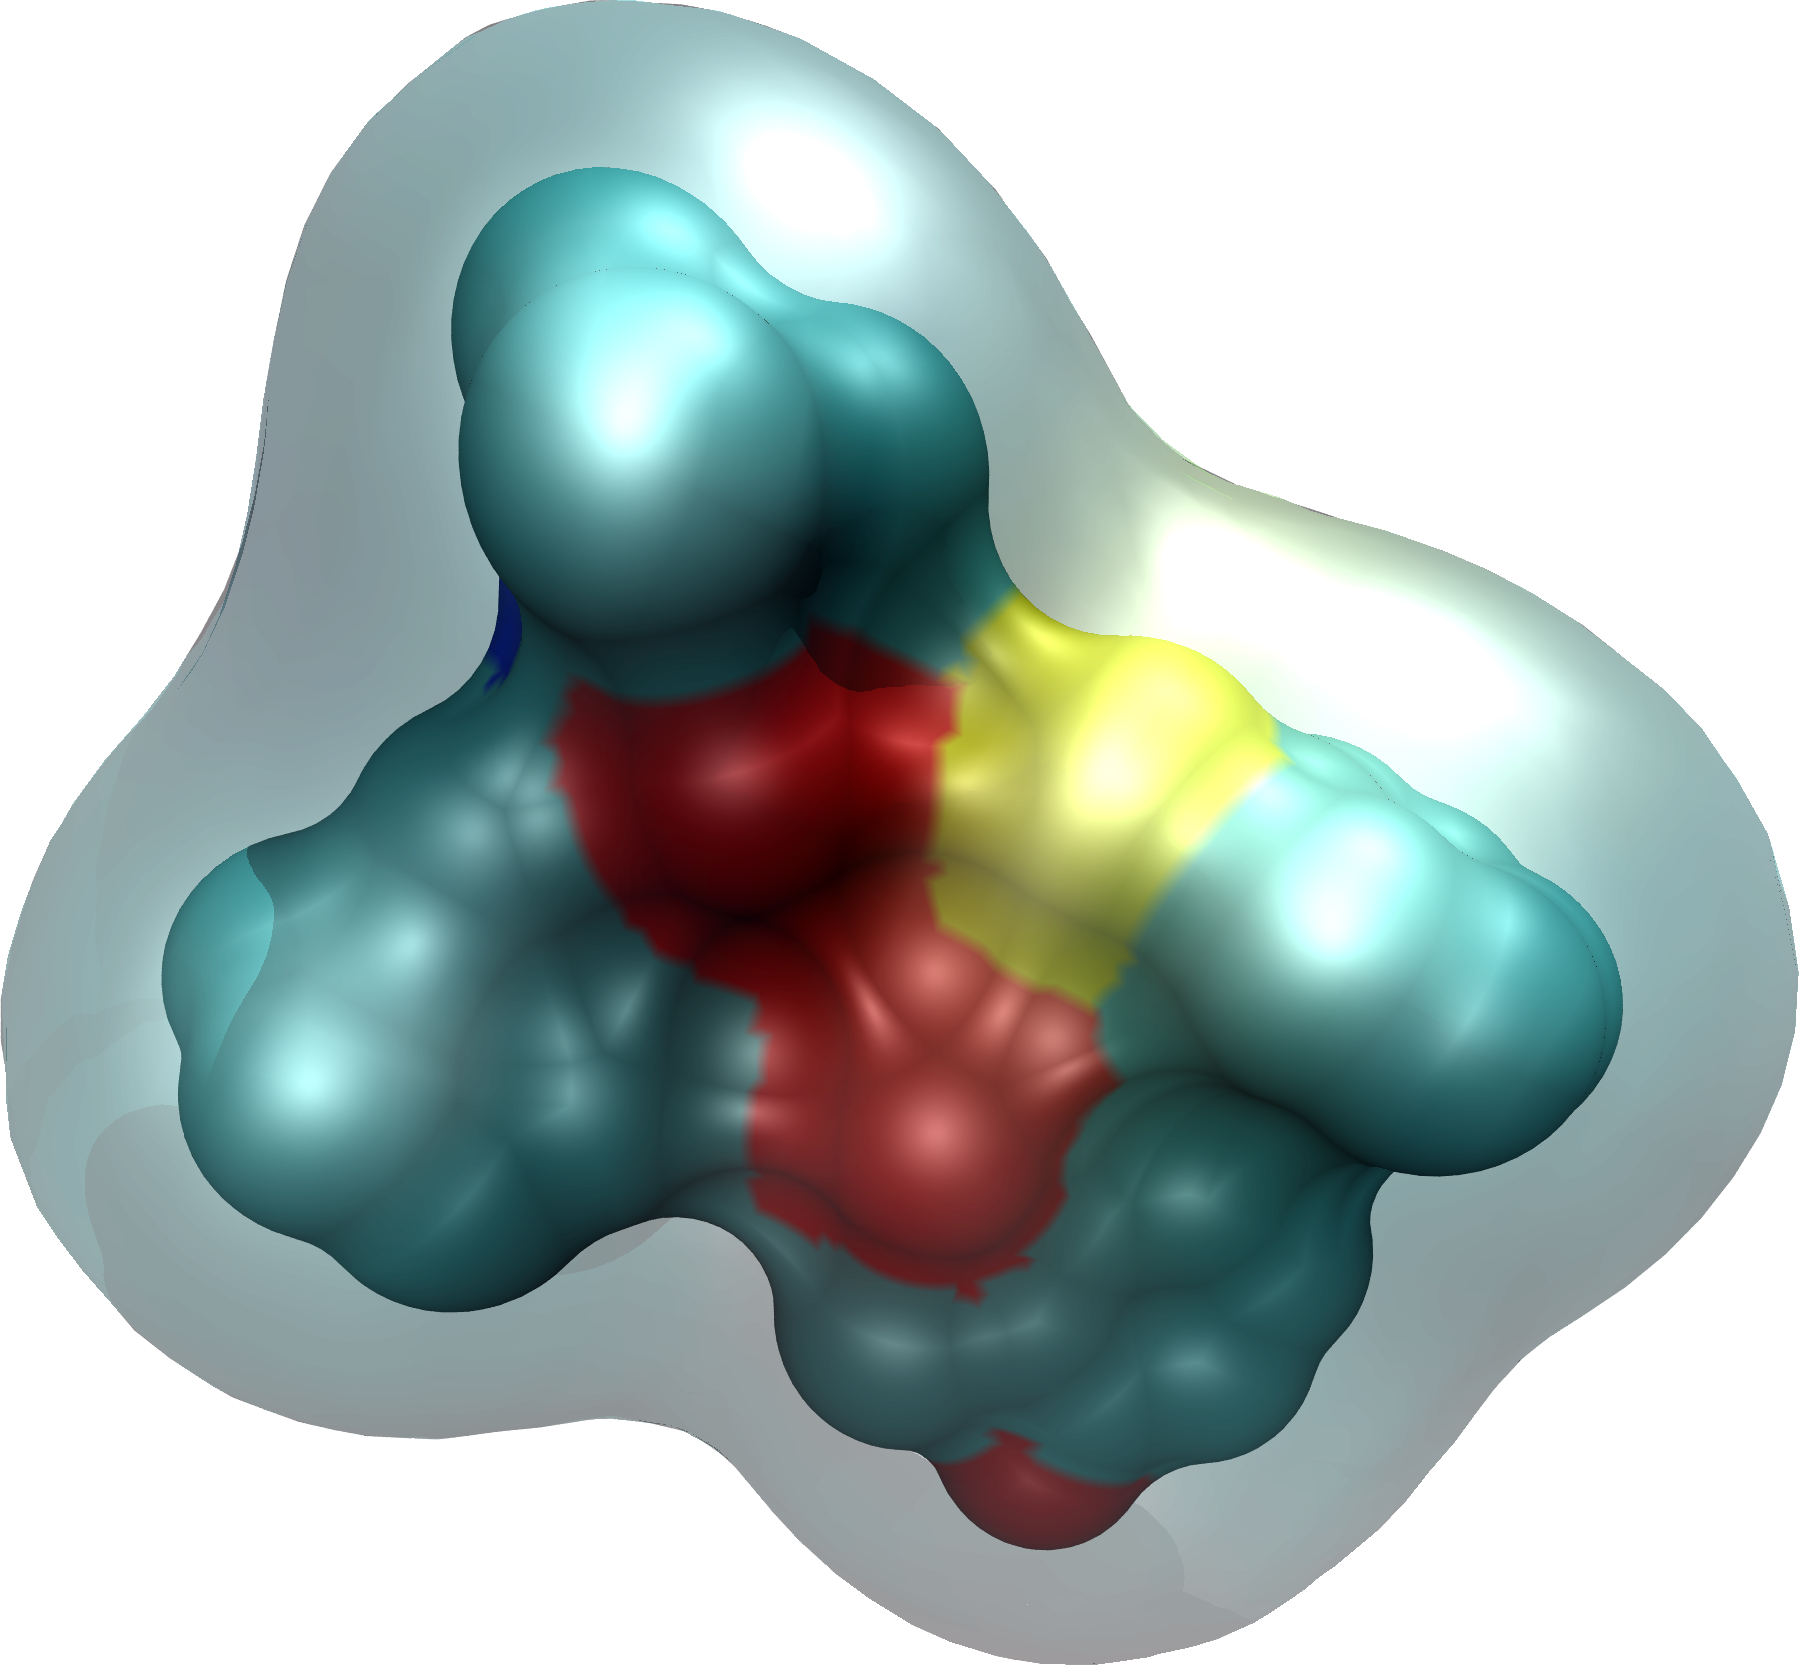
\includegraphics[width=\textwidth]{figures/molecular.png}
\caption{}
\label{figure:molecular_surface}
\end{subfigure}
\caption{(a) The Van der Waals surface of Nelfinavir, defined by the surface of the volume excluded by the VDW radii of the atoms in the structure.
(b) The molecular surface, defined as the surface of the volume excluded from a probe of 1.4 angstroms (the radius of a water molecule).
Both surfaces are enclosed by an approximate solvent accessible surface, which is defined as the surface traced by rolling a spherical probe over the VDW surface.
Figure generated using Nelfinavir structure from PDBid 3EL5 \protect\cite{king2012extreme}, and using VMD and POV-Ray \protect\cite{humphrey1996vmd,povray}.}
\label{figure:surfaces}
\end{figure}
\begin{enumerate}
\item The Van der Waals (VDW) surface is the surface formed by the VDW radius of each molecule, though the exact radii mayy vary in different energy functions.
Frequently the VDW radii are scaled down in order to reduce the effect of steric clashes and help generate more initial structures \cite{schulz2003binding,halgren2004glide}.
Clashes which are tolerated using these scaled down radii can later be resolved in minimization.
This is illustrated in figure \ref{figure:vdw_surface}.
\item The solvent accessible surface, which is defined as the surface traced by the center of a spherical probe ``rolled'' over the VDW surface \cite{richards1977areas}.
This idea is very closely related to the idea of the solvent excluded volume, or the shape of the solvent cavity enforced by the VDW surface of the molecule \cite{richmond1984solvent}.
An illustration of the solvent accessible surface is shown enclosing both a VDW and molecular surface in \ref{figure:surfaces}.
\item The molecular surface, or Connolly surface, is composed of the VDW surface in areas where the spherical probe touches the VDW surface, in union with all points on the probe ``between'' two points on the VDW surface when the probe is contacting multiple atoms \cite{connolly1983analytical} -- put another way, the surface of the volume which intersects no possible probe location.
This is shown in \ref{figure:molecular_surface}
\end{enumerate}
Frequently, these surfaces are approximated numerically, using the Shrake-Rupley algorithm \cite{shrake1973environment}, by considering a spherical mesh about every atom and including only points that satisfy the definition of the surface, or using these points to interpolate a surface.

The effect of surface area on determining protein structure is determined by physical forces.
However, the significance of the effect of surface area is well illustrated by the observation that the ratio of total area of a theoretical unfolded, i.e. linearly arranged, protein to its length is almost among proteins, only varying by \textapprox3\% between different proteins.
